\chapter{Kiểm thử}

\section{Kiểm thử phần mềm và chiến lược kiểm thử}

Kiểm thử phần mềm là quá trình đánh giá và xác minh có hệ thống rằng một ứng dụng
phần mềm thực hiện đúng các chức năng đã định, đáp ứng các yêu cầu kỹ thuật và
không có các lỗi nghiêm trọng~\cite{testing_definition}. Ngoài việc phát hiện lỗi,
kiểm thử phần mềm hiện đại còn đóng vai trò là cơ chế đảm bảo chất lượng, xác nhận
độ tin cậy, tính bảo mật và hiệu năng của hệ thống trong nhiều điều kiện khác nhau.

Để đảm bảo tính ổn định của Hệ thống quản lý thư viện, dự án áp dụng phương pháp
kiểm thử phân tầng. Việc kiểm thử được thực hiện qua nhiều tầng---từ các thành phần
riêng lẻ đến các luồng tích hợp hoàn chỉnh---đảm bảo rằng mỗi tầng của kiến trúc
được xác minh trước khi tiến đến tầng tiếp theo~\cite{test_pyramid}. Các phần tiếp
theo sẽ trình bày chi tiết các chiến lược kiểm thử cụ thể được áp dụng trong dự án.

\subsection{Kiểm thử đơn vị}

Kiểm thử đơn vị (Unit Testing) là tầng kiểm thử đầu tiên, nơi các phần nhỏ nhất
có thể kiểm thử được của ứng dụng---gọi là ``đơn vị''---là các thành phần hoặc hàm
riêng lẻ được cô lập và xác minh tính đúng đắn~\cite{unit_testing}. Bằng cách phát
hiện lỗi ngay ở tầng này, nhóm phát triển đảm bảo rằng logic nghiệp vụ cốt lõi của
ứng dụng luôn ổn định trong suốt quá trình phát triển và tái cấu trúc. Các bài kiểm
thử đơn vị được thiết kế để chạy nhanh và độc lập, với tất cả các phụ thuộc bên
ngoài như cơ sở dữ liệu, message broker và API ngoài được thay thế bằng đối tượng
giả lập (mock).

\subsection{Kiểm thử tích hợp}

Sau khi các đơn vị riêng lẻ được xác minh, kiểm thử tích hợp (Integration Testing)
được thực hiện để đánh giá sự tương tác và luồng dữ liệu giữa các module phần mềm
khác nhau~\cite{integration_testing}. Tầng kiểm thử này tập trung vào giao diện
giữa các thành phần, xác minh rằng các module đã tách rời của hệ thống hoạt động
cùng nhau như một đơn vị thống nhất. Không giống kiểm thử đơn vị, kiểm thử tích hợp
sử dụng hạ tầng thực như cơ sở dữ liệu để xác nhận toàn bộ luồng dữ liệu hoạt động
đúng từ đầu đến cuối.

\subsection{Kiểm thử API}

Kiểm thử API xác nhận hợp đồng giao tiếp giữa frontend và backend bằng cách gửi các
yêu cầu HTTP đến các endpoint REST và kiểm tra mã trạng thái phản hồi, header và
payload JSON~\cite{api_testing}. Hình thức kiểm thử này nằm giữa kiểm thử tích hợp
và kiểm thử hệ thống, xác nhận rằng máy chủ xử lý đúng các tình huống khác nhau---
bao gồm yêu cầu hợp lệ, lỗi xác thực và vi phạm quy tắc nghiệp vụ---mà không cần
giao diện người dùng đầy đủ.

\subsection{Kiểm thử hiệu năng}

Kiểm thử hiệu năng (Performance Testing) đánh giá khả năng phản hồi, tính ổn định
và khả năng mở rộng của hệ thống dưới các tải trọng khác nhau~\cite{performance_testing}.
Nó được sử dụng để xác định các điểm nghẽn trong pipeline xử lý và đảm bảo rằng
các yêu cầu từ nhiều người dùng đồng thời không làm suy giảm trải nghiệm tổng thể.
Các chỉ số chính được thu thập bao gồm thời gian phản hồi trung bình, phân vị thứ
95 (p95), số lượng yêu cầu mỗi giây (RPS) và tỷ lệ lỗi dưới tải.

% ─────────────────────────────────────────────────────────────────────────────
\section{Kiểm thử đơn vị}
% ─────────────────────────────────────────────────────────────────────────────

\subsection{Framework kiểm thử Backend (JUnit 5 + Mockito)}

Đối với kiến trúc backend xây dựng trên Java 21 và Spring Boot 3.3.5, bộ kiểm thử
sử dụng JUnit 5 kết hợp với framework giả lập Mockito.

\subsubsection{JUnit 5}
JUnit 5 là framework kiểm thử tiêu chuẩn cho các ứng dụng Java. Framework cung cấp
tập hợp phong phú các annotation---như \texttt{@Test}, \texttt{@BeforeEach} và
\texttt{@DisplayName}---để cấu trúc việc thực thi kiểm thử, đồng thời tích hợp
liền mạch với vòng đời build Maven thông qua \texttt{maven-surefire-plugin}~\cite{junit5}.

\subsubsection{Mockito}
Mockito là framework giả lập (mocking) cho Java, cho phép tạo và cấu hình các đối
tượng mock, thay thế phụ thuộc thực bằng các thay thế có kiểm soát. Trong dự án
này, Mockito được sử dụng để giả lập \texttt{ItemStatusPort}, \texttt{KafkaTemplate}
và các interface repository, đảm bảo mỗi use case có thể được kiểm thử hoàn toàn
độc lập~\cite{mockito}.

\subsection{Framework kiểm thử Frontend (Jest)}

Đối với kiến trúc frontend xây dựng trên React 19 và TypeScript, bộ kiểm thử sử
dụng Jest kết hợp với bộ chuyển đổi ts-jest.

\subsubsection{Jest}
Jest là framework kiểm thử JavaScript tập trung vào sự đơn giản~\cite{jest}. Nó
đóng vai trò là test runner, thư viện assertion và framework giả lập cốt lõi. Jest
được tối ưu cho môi trường Node.js và thực thi kiểm thử nhanh chóng bằng cách sử
dụng jsdom để mô phỏng môi trường trình duyệt.

\subsubsection{ts-jest}
Do dự án được viết bằng TypeScript, ts-jest được sử dụng như một bộ tiền xử lý biên
dịch các file TypeScript trước khi Jest thực thi. Cấu hình được khai báo trong
\texttt{jest.config.cjs} (định dạng CommonJS, bắt buộc vì \texttt{package.json}
của dự án khai báo \texttt{"type": "module"}).

\subsection{Thiết kế test case}

Các test case trên cả frontend và backend đều tuân thủ nghiêm ngặt mẫu
Arrange-Act-Assert (AAA) để đảm bảo khả năng đọc và bảo trì:

\begin{itemize}
    \item \textbf{Arrange (Chuẩn bị):} Thiết lập trạng thái ban đầu, khởi tạo các
          đối tượng mock và cấu hình giá trị trả về bằng
          \texttt{when(...).thenReturn(...)}.
    \item \textbf{Act (Thực thi):} Gọi phương thức hoặc hàm cụ thể đang được kiểm
          thử.
    \item \textbf{Assert (Kiểm tra):} Xác minh rằng kết quả thực tế khớp với kết
          quả mong đợi bằng AssertJ (backend) hoặc Jest \texttt{expect} (frontend).
\end{itemize}

\subsubsection{Trọng tâm kiểm thử Backend}
Chiến lược kiểm thử backend nhắm vào ba use case nghiệp vụ cốt lõi của module
circulation. Tất cả các phụ thuộc bên ngoài---bao gồm cơ sở dữ liệu thông qua
\texttt{ItemStatusPort}, Kafka message broker thông qua \texttt{KafkaTemplate} và
JPA repository---được tách biệt hoàn toàn bằng Mockito để đảm bảo thực thi xác
định và độc lập với mạng. Mỗi use case được kiểm thử với ít nhất một kịch bản
happy-path và một kịch bản error-path xác nhận việc ném \texttt{AppException} đúng
lỗi.

\subsubsection{Trọng tâm kiểm thử Frontend}
Chiến lược kiểm thử frontend tập trung vào các hàm tiện ích thuần túy (pure
functions) đóng gói logic nghiệp vụ của trang đặt trước, cụ thể là module
\texttt{reservationUtils.ts}. Việc kiểm thử các pure function---những hàm không có
tác dụng phụ hay gọi API bên ngoài---đảm bảo cô lập tối đa và thực thi nhanh.

\subsection{Danh sách test case}

Bảng~\ref{tab:unit_be} tổng hợp các test case kiểm thử đơn vị backend được triển
khai trong module \texttt{library-circulation-module}.

\begin{table}[h]
\centering
\caption{Danh sách test case kiểm thử đơn vị Backend}
\label{tab:unit_be}
\begin{tabular}{|l|p{4cm}|p{4cm}|l|}
\hline
\textbf{Class} & \textbf{Tên test} & \textbf{Kịch bản} & \textbf{Kết quả mong đợi} \\
\hline
\multirow{4}{*}{\texttt{BorrowRequest}}
  & borrowSuccess & Item AVAILABLE, không có fine & WAITING\_FOR\_PICKUP \\
\cline{2-4}
  & itemNotAvailable & Item đang ở trạng thái BORROWED & AppException \\
\cline{2-4}
  & unpaidFines & User có khoản phạt chưa thanh toán & AppException \\
\cline{2-4}
  & duplicateBorrow & Cùng ấn phẩm đang được mượn & AppException \\
\hline
\multirow{3}{*}{\texttt{ReturnBook}}
  & returnSuccess\_noFine & Trả trước hạn & RETURNED, không tạo fine \\
\cline{2-4}
  & returnSuccess\_withFine & Trả trễ 3 ngày & Fine = 3.000 VNĐ \\
\cline{2-4}
  & transactionNotFound & Không có giao dịch đang mượn & AppException \\
\hline
\multirow{5}{*}{\texttt{CreateReservation}}
  & reservationSuccess & Item không có sẵn, không có fine & PENDING \\
\cline{2-4}
  & unpaidFines & User có khoản phạt chưa thanh toán & AppException \\
\cline{2-4}
  & limitExceeded & Đã có 2 đặt trước đang hoạt động & AppException \\
\cline{2-4}
  & itemAvailable & Item đang AVAILABLE tại cơ sở & AppException \\
\cline{2-4}
  & duplicateReservation & Đã đặt trước ấn phẩm này & AppException \\
\hline
\end{tabular}
\end{table}

Bảng~\ref{tab:unit_fe} tổng hợp các test case kiểm thử đơn vị frontend được triển
khai trong \texttt{reservationUtils.test.ts}.

\begin{table}[h]
\centering
\caption{Danh sách test case kiểm thử đơn vị Frontend}
\label{tab:unit_fe}
\begin{tabular}{|l|p{6cm}|c|}
\hline
\textbf{Nhóm} & \textbf{Tên test} & \textbf{Kết quả} \\
\hline
\multirow{6}{*}{\texttt{STATUS\_CONFIG}}
  & Hiển thị đúng nhãn cho trạng thái PENDING & Pass \\
\cline{2-3}
  & Hiển thị đúng màu cho trạng thái READY\_FOR\_PICKUP & Pass \\
\cline{2-3}
  & Hiển thị đúng nhãn cho trạng thái BORROWING & Pass \\
\cline{2-3}
  & Hiển thị đúng nhãn cho trạng thái COMPLETED & Pass \\
\cline{2-3}
  & Hiển thị đúng nhãn cho trạng thái CANCELLED & Pass \\
\cline{2-3}
  & Hiển thị đúng nhãn cho trạng thái OVERDUE & Pass \\
\hline
\multirow{3}{*}{\texttt{fmtDate}}
  & Định dạng đúng chuỗi ngày ISO hợp lệ & Pass \\
\cline{2-3}
  & Trả về gạch ngang khi đầu vào là null & Pass \\
\cline{2-3}
  & Trả về gạch ngang khi đầu vào là undefined & Pass \\
\hline
\multirow{5}{*}{\texttt{isActiveCancellable}}
  & Trả về true cho trạng thái PENDING & Pass \\
\cline{2-3}
  & Trả về true cho trạng thái READY\_FOR\_PICKUP & Pass \\
\cline{2-3}
  & Trả về false cho trạng thái COMPLETED & Pass \\
\cline{2-3}
  & Trả về false cho trạng thái CANCELLED & Pass \\
\cline{2-3}
  & Trả về false cho trạng thái EXPIRED & Pass \\
\hline
\multirow{4}{*}{\texttt{calcHoldDeadlineLabel}}
  & Trả về số giờ còn lại khi còn hơn 1 giờ & Pass \\
\cline{2-3}
  & Trả về ``sắp hết hạn'' khi còn dưới 1 giờ & Pass \\
\cline{2-3}
  & Trả về ``đã hết hạn'' khi quá thời hạn & Pass \\
\cline{2-3}
  & Trả về gạch ngang khi deadline là null & Pass \\
\hline
\end{tabular}
\end{table}

\subsection{Kết quả}

Bộ kiểm thử đơn vị tự động cho cả frontend và backend đã được thực thi thành công,
thể hiện tính ổn định cao của logic nghiệp vụ cốt lõi trong hệ thống.

\subsubsection{Kết quả Backend}
Kiểm thử đơn vị backend xác nhận ba use case circulation chính trong môi trường hoàn
toàn cô lập. Tất cả phụ thuộc bên ngoài được giả lập hoàn toàn bằng Mockito để
đảm bảo thực thi xác định.

\begin{itemize}
    \item Tổng số class kiểm thử: 3
    \item Tổng số test case: 12
    \item Passed: 12
    \item Failed: 0
    \item Thời gian thực thi: $\approx$4 giây
\end{itemize}

\begin{figure}[h]
    \centering
    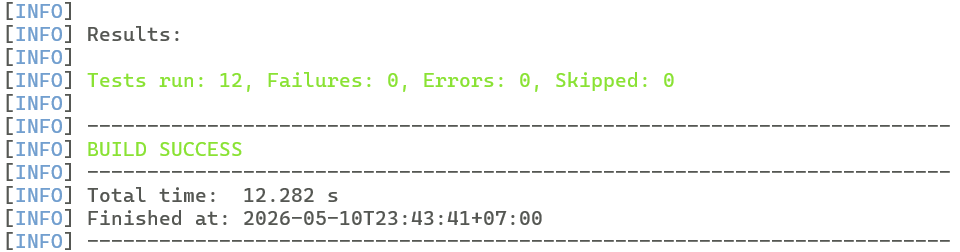
\includegraphics[width=0.9\textwidth]{figures/unit_test_be_result.png}
    \caption{Kết quả kiểm thử đơn vị Backend
             (\texttt{mvn test -pl library-circulation-module})}
    \label{fig:unit_be_result}
\end{figure}

\subsubsection{Kết quả Frontend}
Kiểm thử đơn vị frontend xác nhận các hàm tiện ích đặt trước đóng gói logic nghiệp
vụ UI quan trọng.

\begin{itemize}
    \item Tổng số test suite: 1
    \item Tổng số test case: 18
    \item Passed: 18
    \item Failed: 0
    \item Thời gian thực thi: $\approx$2.3 giây
\end{itemize}

\begin{figure}[h]
    \centering
    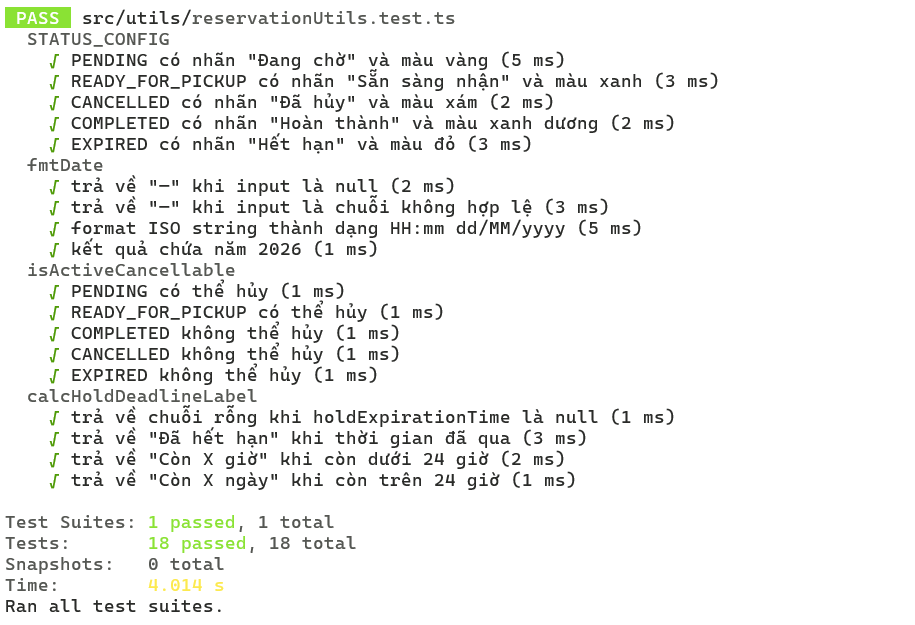
\includegraphics[width=0.9\textwidth]{figures/unit_test_fe_result.png}
    \caption{Kết quả kiểm thử đơn vị Frontend (\texttt{npm test})}
    \label{fig:unit_fe_result}
\end{figure}

% ─────────────────────────────────────────────────────────────────────────────
\section{Kiểm thử tích hợp}
% ─────────────────────────────────────────────────────────────────────────────

\subsection{Chiến lược kiểm thử}

Chiến lược kiểm thử tích hợp cho backend tập trung vào việc xác nhận toàn bộ
vòng đời mượn-trả sách qua tất cả các tầng hạ tầng thực---bao gồm cơ sở dữ liệu
PostgreSQL, tầng persistence JPA và các use case domain---trong khi cô lập các
dịch vụ bên thứ ba không liên quan đến luồng nghiệp vụ đang kiểm thử.

\subsubsection{SpringBootTest và Testcontainers}
Class kiểm thử được đánh dấu với \texttt{@SpringBootTest(webEnvironment = NONE)},
khởi động đầy đủ application context của Spring mà không khởi chạy HTTP server.
Điều này cho phép inject trực tiếp các bean use case và JPA repository trong khi
vẫn giữ tốc độ thực thi. Một instance PostgreSQL 15 thực sự được cung cấp theo
yêu cầu bằng Testcontainers~\cite{testcontainers}---một thư viện Java quản lý
container Docker trong vòng đời JUnit. URL kết nối cơ sở dữ liệu được inject động
qua \texttt{@DynamicPropertySource}, ghi đè cấu hình datasource production cho
profile kiểm thử.

\subsubsection{Cô lập các dịch vụ bên ngoài}
Các dịch vụ không thuộc phạm vi kiểm thử được thay thế bằng các instance
\texttt{@MockBean} để ngăn kết nối mạng và tác dụng phụ ngoài ý muốn:

\begin{itemize}
    \item \texttt{KafkaTemplate} và \texttt{KafkaAdmin} --- ngăn kết nối đến
          Kafka broker.
    \item \texttt{S3Client} và \texttt{S3Presigner} --- ngăn AWS SDK xác thực
          thông tin đăng nhập.
    \item \texttt{ClientRegistrationRepository} --- ngăn tải cấu hình OAuth2
          provider.
    \item Bốn bean scheduler --- ngăn các background job can thiệp vào kết quả
          kiểm thử.
\end{itemize}

\subsubsection{Cô lập kiểm thử qua \texttt{@BeforeEach}}
Để đảm bảo mỗi phương thức kiểm thử bắt đầu từ trạng thái sạch đã biết trước,
một phương thức setup \texttt{@BeforeEach} thực hiện các thao tác SQL sau trên cơ
sở dữ liệu kiểm thử:

\begin{enumerate}
    \item Xóa tất cả khoản phạt liên quan đến người dùng kiểm thử (ràng buộc
          khóa ngoại yêu cầu thứ tự này).
    \item Xóa tất cả giao dịch mượn sách không ở trạng thái \texttt{RETURNED}
          của người dùng kiểm thử để đặt lại số lượng mượn đang hoạt động.
    \item Xóa tất cả đặt trước \texttt{PENDING} cho ấn phẩm kiểm thử để ngăn
          dịch vụ gán sách tự động sau thao tác trả sách.
    \item Đặt lại trạng thái item kiểm thử về \texttt{AVAILABLE}.
\end{enumerate}

\subsection{Thiết kế test case}

Bộ kiểm thử tích hợp bao gồm vòng đời mượn-trả hoàn chỉnh của Hệ thống quản lý
thư viện, được triển khai trong class \texttt{BorrowFlowIntegrationTest}. Dữ liệu
kiểm thử được seed bởi migration Flyway \texttt{V2\_\_seed\_data.sql}, khởi tạo
người dùng, ấn phẩm, items và các giao dịch mẫu trước khi application context được
tải.

\begin{table}[h]
\centering
\caption{Danh sách test case kiểm thử tích hợp --- Luồng mượn sách}
\label{tab:integration_tests}
\begin{tabular}{|c|p{3cm}|p{4.5cm}|p{3.5cm}|}
\hline
\textbf{Thứ tự} & \textbf{Tên test} & \textbf{Kịch bản} & \textbf{Kết quả mong đợi} \\
\hline
T1 & borrow\_should CreateTransaction AndReserveItem
   & Người dùng đặt mượn một item đang AVAILABLE, không có khoản phạt
   & Transaction = \texttt{WAITING\_FOR\_PICKUP}; Item = \texttt{RESERVED} \\
\hline
T2 & return\_should MarkTransaction ReturnedAndFreeItem
   & Thủ thư trả sách đang \texttt{BORROWING} theo barcode trước hạn
   & Transaction = \texttt{RETURNED}; Item = \texttt{AVAILABLE} \\
\hline
T3 & borrow\_shouldFail\_ whenUserHasUnpaid FineInDB
   & Người dùng cố mượn khi có khoản phạt \texttt{UNPAID} trong DB
   & Ném \texttt{AppException}; không tạo giao dịch mới \\
\hline
\end{tabular}
\end{table}

\subsection{Kết quả}

Bộ kiểm thử tích hợp đã thực thi thành công, xác nhận rằng use case mượn sách,
use case trả sách và quy tắc nghiệp vụ chặn mượn khi có phạt tương tác đúng đắn
với cơ sở dữ liệu PostgreSQL thực.

\begin{itemize}
    \item Tổng số test case: 3
    \item Passed: 3
    \item Failed: 0
    \item Thời gian thực thi: $\approx$37 giây (bao gồm thời gian khởi động
          Testcontainers)
\end{itemize}

\begin{figure}[h]
    \centering
    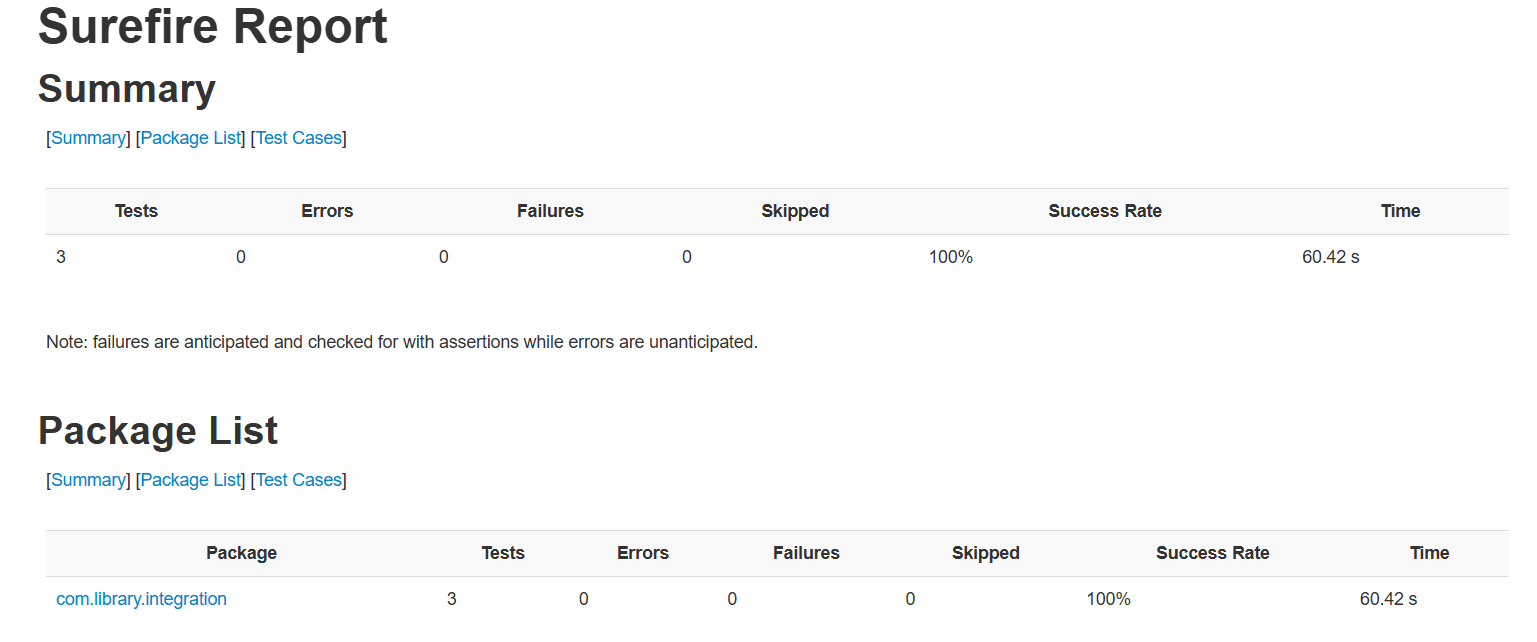
\includegraphics[width=0.9\textwidth]{figures/integration_test_result.png}
    \caption{Kết quả kiểm thử tích hợp --- Surefire HTML Report
             (\texttt{library-bootstrap/target/reports/surefire.html})}
    \label{fig:integration_result}
\end{figure}

% ─────────────────────────────────────────────────────────────────────────────
\section{Kiểm thử API}
% ─────────────────────────────────────────────────────────────────────────────

\subsection{Giới thiệu công cụ}

Postman là nền tảng kiểm thử API phổ biến cung cấp giao diện đồ họa trực quan
để soạn thảo, gửi và kiểm tra các yêu cầu HTTP~\cite{postman}. Postman cho phép
tổ chức các request thành Collection có cấu trúc, định nghĩa biến môi trường
dùng chung và viết script kiểm tra JavaScript tự động sau mỗi request. Tính năng
\textbf{Collection Runner} của Postman cho phép thực thi toàn bộ collection theo
thứ tự, tự động truyền giá trị giữa các request thông qua biến môi trường, và
hiển thị báo cáo tổng hợp kết quả passed/failed ngay trong giao diện.

\subsection{Bộ test collection}

Bộ test collection được tổ chức thành tám thư mục, mỗi thư mục đại diện cho một
luồng API riêng biệt của Hệ thống quản lý thư viện. Bảng~\ref{tab:postman_collection}
trình bày phạm vi kiểm thử của từng thư mục.

\begin{table}[h]
\centering
\caption{Tổng quan Postman Collection}
\label{tab:postman_collection}
\begin{tabular}{|l|c|p{6.5cm}|}
\hline
\textbf{Thư mục} & \textbf{Số request} & \textbf{Nội dung kiểm tra} \\
\hline
00 - Xác thực & 2 & Đăng nhập student + librarian, token lưu vào biến môi trường \\
\hline
01 - Ấn phẩm (công khai) & 4 & Tìm kiếm, sách mới nhất, chi tiết, danh sách item AVAILABLE \\
\hline
02 - Luồng mượn sách & 4 & Đặt mượn (201), tra cứu (200), xác nhận lấy sách (200), lịch sử \\
\hline
03 - Luồng trả sách & 2 & Tra cứu giao dịch đang mượn theo barcode, trả sách \\
\hline
04 - Luồng đặt trước & 3 & Tạo đặt trước (201), danh sách (200), hủy (200) \\
\hline
05 - Quản lý phạt & 1 & Xem danh sách phạt của sinh viên hiện tại \\
\hline
06 - Dashboard & 2 & Tổng hợp dashboard, biểu đồ theo tuần \\
\hline
07 - Trường hợp lỗi & 2 & Mượn không có token (401), đăng nhập sai mật khẩu (4xx) \\
\hline
\textbf{Tổng} & \textbf{20} & \\
\hline
\end{tabular}
\end{table}

Mỗi request bao gồm một script kiểm tra JavaScript trong tab \texttt{Tests} để
xác nhận mã trạng thái HTTP và kiểm tra các trường quan trọng trong body JSON
phản hồi. Các biến môi trường (\texttt{studentToken}, \texttt{librarianToken},
\texttt{transactionId}, \texttt{reservationId}, \texttt{itemId}) được tự động
truyền giữa các request thông qua \texttt{pm.environment.set()}, cho phép
collection thực thi như một luồng tuần tự có trạng thái mà không cần can thiệp
thủ công.

\subsection{Kết quả}

Postman Collection được thực thi trực tiếp trong giao diện Postman thông qua
tính năng \textbf{Collection Runner} với máy chủ backend đang chạy cục bộ tại
\texttt{http://localhost:8080}. Tất cả 20 request được thực thi theo thứ tự,
kết quả kiểm tra hiển thị trực tiếp trong giao diện Runner.

\begin{figure}[h]
    \centering
    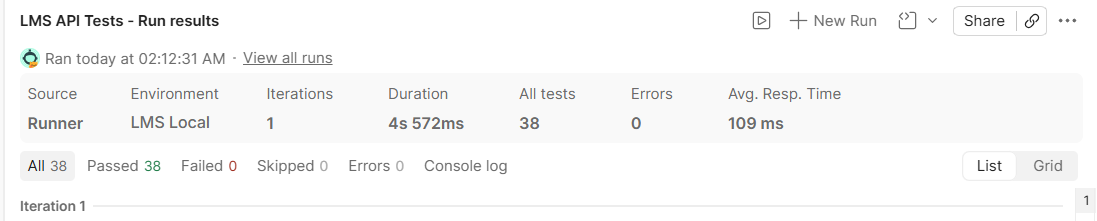
\includegraphics[width=0.9\textwidth]{figures/postman_result.png}
    \caption{Kết quả kiểm thử API --- Postman Collection Runner}
    \label{fig:postman_result}
\end{figure}

% ─────────────────────────────────────────────────────────────────────────────
\section{Kiểm thử hiệu năng}
% ─────────────────────────────────────────────────────────────────────────────

\subsection{Giới thiệu công cụ}

k6 là công cụ kiểm thử hiệu năng mã nguồn mở được viết bằng Go, được thiết kế để
lập trình các kịch bản kiểm thử tải bằng JavaScript~\cite{k6}. Công cụ hỗ trợ
định nghĩa các người dùng ảo (Virtual Users - VU) thực thi các kịch bản kiểm thử
đồng thời, phù hợp để đánh giá hành vi của REST API dưới tải đồng thời thực tế.
k6 tự động báo cáo các chỉ số hiệu năng quan trọng bao gồm phân vị thời gian phản
hồi, thông lượng (RPS) và tỷ lệ lỗi.

\subsection{Cấu hình kiểm thử}

Kiểm thử hiệu năng nhắm vào ba endpoint công khai được truy cập thường xuyên nhất
của hệ thống: API tìm kiếm ấn phẩm, API lấy danh sách sách mới nhất và API sách
được mượn nhiều nhất. Các endpoint này được kỳ vọng chịu tải đọc cao nhất trong
môi trường thư viện thực tế, vì chúng không yêu cầu xác thực và được gọi mỗi
khi người dùng tải trang chủ hoặc trang tìm kiếm công khai.

Kiểm thử được cấu hình theo mô hình ramp-up với ba giai đoạn:

\begin{itemize}
    \item \textbf{Warm-up (10 giây):} Tăng dần từ 0 lên 5 VU để làm nóng hệ thống.
    \item \textbf{Load (20 giây):} Duy trì 10 VU đồng thời --- tải chính của bài kiểm thử.
    \item \textbf{Cool-down (10 giây):} Giảm dần về 0 VU.
    \item \textbf{Thời gian chờ:} 1 giây giữa mỗi lần lặp của mỗi VU.
    \item \textbf{Ngưỡng chấp nhận (thresholds):}
    \begin{itemize}
        \item \texttt{http\_req\_duration p(95) \textless{} 1000ms} --- 95\% yêu cầu hoàn
              thành trong vòng 1 giây.
        \item \texttt{http\_req\_failed rate \textless{} 5\%} --- Tỷ lệ lỗi dưới 5\%.
        \item \texttt{search\_duration p(90) \textless{} 800ms} --- 90\% yêu cầu tìm kiếm
              hoàn thành trong 800ms.
        \item \texttt{newest\_duration p(90) \textless{} 500ms} --- 90\% yêu cầu sách mới
              hoàn thành trong 500ms.
    \end{itemize}
\end{itemize}

\subsection{Kết quả}

Kiểm thử tải k6 được thực thi với máy chủ backend đang chạy cục bộ bằng lệnh:

\begin{verbatim}
k6 run tests/performance/search_load_test.js
\end{verbatim}

Bảng~\ref{tab:k6_results} tổng hợp các chỉ số hiệu năng thu thập được trong
toàn bộ 40 giây kiểm thử (113 iterations, 339 HTTP requests).

\begin{table}[h]
\centering
\caption{Kết quả kiểm thử hiệu năng k6}
\label{tab:k6_results}
\begin{tabular}{|l|c|c|c|}
\hline
\textbf{Chỉ số} & \textbf{Kết quả} & \textbf{Ngưỡng} & \textbf{Trạng thái} \\
\hline
Thời gian phản hồi trung bình & 5.53 ms   & ---       & --- \\
\hline
Phân vị p90                   & 6.49 ms   & ---       & --- \\
\hline
Phân vị p95                   & 7.08 ms   & $<$ 1000ms  & \textbf{Đạt} \checkmark \\
\hline
Số yêu cầu mỗi giây (RPS)     & 8.30 req/s & ---      & --- \\
\hline
Tỷ lệ lỗi HTTP                & 0.00\%    & $<$ 5\%     & \textbf{Đạt} \checkmark \\
\hline
Kiểm tra (checks)             & 100\%     & ---       & \textbf{Đạt} \checkmark \\
\hline
\end{tabular}
\end{table}

Kết quả cho thấy hệ thống xử lý tốt tải đồng thời 10 người dùng với thời gian
phản hồi trung bình chỉ 5.53ms và tỷ lệ lỗi 0\%. Tất cả 5 ngưỡng chấp nhận
(thresholds) đều đạt yêu cầu, xác nhận hiệu năng của các API công khai đáp ứng
tiêu chuẩn vận hành trong điều kiện thực tế.

\begin{figure}[h]
    \centering
    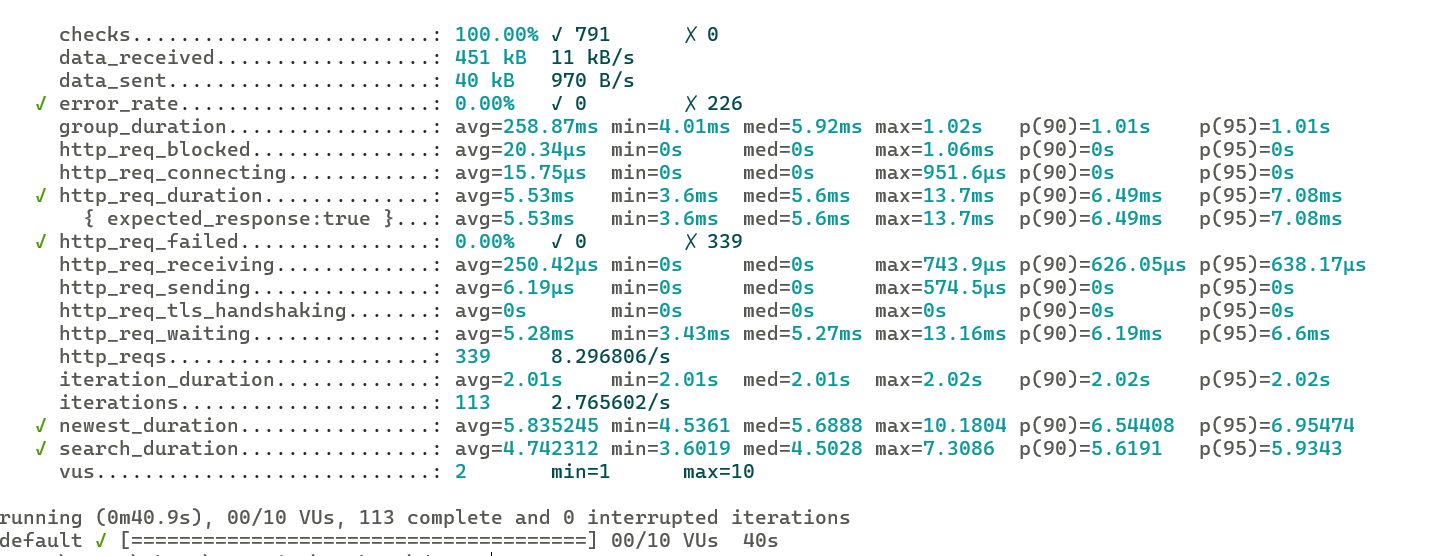
\includegraphics[width=0.9\textwidth]{figures/k6_result.png}
    \caption{Kết quả kiểm thử hiệu năng k6 --- tất cả thresholds đạt yêu cầu}
    \label{fig:k6_result}
\end{figure}

% ─────────────────────────────────────────────────────────────────────────────
\section{Tổng kết}
% ─────────────────────────────────────────────────────────────────────────────

Chiến lược kiểm thử được áp dụng trong dự án bao gồm bốn tầng bổ sung cho nhau,
cùng xác nhận tính đúng đắn, tích hợp, hợp đồng API và đặc tính hiệu năng của
Hệ thống quản lý thư viện. Bảng~\ref{tab:test_summary} cung cấp tổng quan tổng hợp
về tất cả kết quả kiểm thử.

\begin{table}[h]
\centering
\caption{Tổng hợp kết quả kiểm thử}
\label{tab:test_summary}
\begin{tabular}{|l|l|c|c|c|}
\hline
\textbf{Loại kiểm thử} & \textbf{Công cụ} & \textbf{Tổng} & \textbf{Passed} & \textbf{Failed} \\
\hline
Kiểm thử đơn vị (BE) & JUnit 5 + Mockito          & 12  & 12  & 0 \\
\hline
Kiểm thử đơn vị (FE) & Jest + ts-jest             & 18  & 18  & 0 \\
\hline
Kiểm thử tích hợp    & SpringBootTest + Testcontainers & 3 & 3 & 0 \\
\hline
Kiểm thử API         & Postman Collection Runner  & 20  & 20  & 0  \\
\hline
Kiểm thử hiệu năng   & k6                         & \multicolumn{3}{c|}{Xem Bảng~\ref{tab:k6_results}} \\
\hline
\end{tabular}
\end{table}

Các bài kiểm thử đơn vị backend và frontend tự động, cùng với bộ kiểm thử tích hợp,
đạt tổng cộng 33 test case tự động với tỷ lệ pass 100\%. Các kết quả này xác nhận
tính ổn định của logic nghiệp vụ cốt lõi---cụ thể là luồng đặt mượn sách, trả sách
và tạo đặt trước---và cho thấy kiến trúc Spring Boot đa module lưu trữ đúng đắn
trạng thái domain vào cơ sở dữ liệu PostgreSQL thực.

Bộ test collection Postman gồm 20 request tổ chức thành 8 luồng chức năng xác nhận
toàn bộ hợp đồng HTTP giữa client và server. Kiểm thử hiệu năng k6 với 10 người dùng
ảo đồng thời cho thấy thời gian phản hồi trung bình 5.53ms và tỷ lệ lỗi 0\%, tất cả
ngưỡng chấp nhận đều đạt yêu cầu. Cùng nhau, bốn tầng kiểm thử này tạo thành một
khung đảm bảo chất lượng toàn diện, phù hợp với một hệ thống quản lý thư viện sẵn
sàng đưa vào môi trường sản xuất.
